\documentclass[11pt, onecolumn]{article}
% \setlength{\columnsep}{0.2cm}

\usepackage{amssymb}
\usepackage{amsmath}
\usepackage[a4paper, margin=2.5cm]{geometry}
%\usepackage{mathtools}
\usepackage{graphicx}

\usepackage[colorlinks=true,linkcolor=blue]{hyperref}
%\hypersetup{ pdfborder = {0 0 0}}

\usepackage{color}
\usepackage[usenames,dvipsnames,svgnames,table]{xcolor}

\usepackage[parfill]{parskip}
\title{Documentation on STI agent model}
\author{David Champredon}

\newcommand{\ttt}[1]{\texttt{#1}}
\newcommand{\one}[1]{\textbf{\large{1}}_{#1}}
\newcommand{\warning}[1]{\textbf{\textcolor{OrangeRed}{#1}}}
\newcommand{\note}[1]{\textit{\textcolor{Grey}{Note: #1}}}

\begin{document}
\maketitle

\tableofcontents


%%%%%%%%%%%%%%%%%%%%%%%%%%%%%%%%%%%%%%%%%%%%%%%%
%%%%%%%%%%%%%%%%%%%%%%%%%%%%%%%%%%%%%%%%%%%%%%%%
\newpage

\section{Introduction and Summary}

This documentation describes the implementation of a stochastic individual based epidemiological model that studies specifically sexually transmitted infections (STIs). A particular aim of this model is its ability to simulate epidemics of several concomitant STIs.

This model attempts to represent fairly realistically three dynamics:
\begin{itemize}
\item \textbf{Demography:} Some infections (e.g., HIV,HSV2, Syphilis) have an infectious period that lasts years if not decades. So, unlike other diseases (e.g., influenza) where the demographic changes over the epidemic period could be neglected, here it is important to have a good representation of the ageing processes of the population (growth rates but also age distribution). Individuals are simulated from the age of sexual debut (for example 12 years old) to an age where sexual activity is very unlikely (`maximum age', for example 80 years old). The `birth' process is actually a recruitment of young (at the predetermined sexual debut age) individuals. Death can occur naturally or is disease induced (both distributed as Weibull). When an individual reaches the maximum age (80 years), death is provoked. 

\item \textbf{Sexual activity:} The contact pattern for STI transmission is driven by partnership formation/dissolution and the rate of sex acts. Individuals can have multiple concurrent partners. Spousal partnerships are also modelled: they are a non-negligible fraction of all partnerships and their formation/dissolution process is distinctive from casual ones. The decision to form or dissolve any partnership is based on simple rules based on age, current number of partners, symptomatic status of potential STI infections and risk group. 
There are three risk group for the general population: low, medium and high-risk. Individuals belonging to a given risk group will be assigned representative parameter values associated with their risk behavior (e.g., use of condom, number of concurrent partners, partner switch rates). High activity commercial sex workers (engaging with multiple partners in a very short period of time) form a fourth distinct risk group which is not included in the partnership formation process (only sex acts are recorded).
The rate and type of sex acts are distributed randomly based on several variables (e.g., age, spousal status, number of concurrent partners, symptomatic status, etc).

\item \textbf{Disease transmission:} Once the network of partnership is built following the demographic and partnerships processes, diseases can spread through its edges. STIs have very different infectious features: probability of transmission per sex act, infectious period and recurrence frequency can vary of orders of magnitudes. Hence, each STI is represented with its own infectivity curve (probability of transmission with respect to time). Because the focus of this model is on STIs co-infections, there are adjusting coefficients on the level of the infectivity curve simulating a potential increase in infectiousness from an individual carrying other STIs. Likewise, susceptibility to STIs varies with potential co-infections.

\end{itemize}

The simulations are run in three steps. First, it starts from an initial population with no partnerships and the model runs for a long enough time (e.g. 50 years with a coarse time step) to match target levels on demography (for example growth rate and age distribution) and partnerships (fraction of single individuals, fraction of spousal partnerships). This is the pre-epidemic era where the model should reach its equilibrium values.

The second step introduces STIs in the population. The sexual activity and disease transmission parameters are calibrated on target prevalences. The model is run for a long enough time with a fine time step, in order to have a good fit with target prevalences of the epidemic era. 

The third step is the analysis and/or prediction. Simulations are run with intervention strategies and/or introduction of a new STI.

There is no migration in or out the population (apart from recruitment of commercial sex workers)

The model is implemented in C++ and wrapped in a R library. Computing power is critical when the population is large and the time horizon long (typically more than 10,000 individuals for more than 10 years with a time step shorter than a week), so a basic parallel implementation is used. 


%%%%%%%%%%%%%%%%%%%%%%%%%%%%%%%%%%%%%%%%%%%%%
%%%%%%%%%%%%%%%%%%%%%%%%%%%%%%%%%%%%%%%%%%%%%
%%%%%%%%%%%%%%%%%%%%%%%%%%%%%%%%%%%%%%%%%%%%%


\section{Individuals, Population and STI}

There are three main class of objects: \ttt{Individual}, \ttt{Population} and \ttt{STI}.

In this individuals based model, a distinction is made between attributes at the `atomic' individual (i.e. age) and the ones that belong to the population (i.e. maximum partnership formation rate). 

An individual is mainly characterized by biological and social features (not exhaustive list): 
\begin{itemize}
\item biological: gender, age, STI infections
\item social: risk group, number of partnerships, marital status
\end{itemize}

A population is characterized by a vector of individuals, a vector of STIs and other scalar parameters (like, for example, the maximum rate of partnership formation).

STIs objects describe the key features of the natural history of the infection. It is independent of individuals or populations.



%%%%%%%%%%%%%%%%%%%%%%%%%%%%%%%%%%%%%%%%%%%%%
%%%%%%%%%%%%%%%%%%%%%%%%%%%%%%%%%%%%%%%%%%%%%
%%%%%%%%%%%%%%%%%%%%%%%%%%%%%%%%%%%%%%%%%%%%%

\section{Demographics}

\subsection{Birth}

Births are modelled as `youth arrival' and allocated to females that are able to be pregnant (i.e. age in a pre-defined range, must be in a partnership and not already pregnant). Young individuals just turning the minimum age of sexual activity enter randomly the population. The expected rate of arrival is 
$$ \alpha = \mathrm{birthRate}\times(1-m_\mathrm{infant})(1-m_{\mathrm{child}})^4 (1-m_{\mathrm{child}}/2)^{n_{min}-5} $$
with $m_\mathrm{infant}$ the mortality rate of infant ($<1$ year-old), $m_\mathrm{child}$ the mortality rate of children $<5$ years-old and $n_{min}$ the minimum age of sexual activity (it is assumed the mortality rate for children between 5 and $n_{min}$ is half).

Then, the number $N$ of youth (aged $n_{min}$ years-old) arrivals during a given period of time $dt$, for a population of size $T$, is:
$$ N \sim \mathrm{Poisson} ( \alpha \, T \,dt)$$


\subsection{Death}

The classical methodology of survival analysis is applied here. The probability of dying between this time step and the previous one is assessed for every individual, at every time step. The probability driving this process is based on 
$$\Pr(t<T_{\mathrm{death}}<t+dt \ | \ T_{\mathrm{death}}\geq t) = \frac{F(t+dt)-F(t)}{1-F(t)}$$
where $T_{\mathrm{death}}$ is the time of death and $F$ its cumulative distribution function. It is assumed that the survival time is Weibull distributed, so the associated hazard function $h$  is given by
\begin{eqnarray}
h(t) &=& \lim_{dt\to 0}\Pr(t<T_{\mathrm{death}}<t+dt \ | \ T_{\mathrm{death}}\geq t)/dt \\
 & =& k\lambda(\lambda t)^{k-1}
\end{eqnarray}
for $k>0$ and $\lambda>0$ the standard Weibull shape and scale parameters, and $t$ the age of the individual. 

If $t_{HIV}$ is the time when the individual was infected with HIV, the hazard function changes and is now parameterized with new shape and scale parameters, and duration since infection instead of age:
$$h_{HIV}(t) = k'\lambda'(\lambda' (t-t_{HIV}))^{k'-1}$$

This probability has to be evaluated at every time step, for every individuals. An example of a plot of this hazard function is illustrated in Figure \ref{fig:deathHazard}.

\begin{figure}[!ht]
\centering
    \includegraphics[angle=0,width=0.9\textwidth]{figures/hazard_death.pdf}
\caption{Death hazard. The red dot represents the age of HIV acquisition. Vertical dashed lines are set at 5, 7 and 10 years after HIV acquisition.}
\label{fig:deathHazard}
\end{figure}


%%%%%%%%%%%%%%%%%%%%%%%%%%%%%%%%%%%%%%%%%%%%%
%%%%%%%%%%%%%%%%%%%%%%%%%%%%%%%%%%%%%%%%%%%%%
%%%%%%%%%%%%%%%%%%%%%%%%%%%%%%%%%%%%%%%%%%%%%



\section{Partnerships}

%[[TO DO: BE EXPLICIT ABOUT RATE OF MATCHING FOR ANY PAIR, AND UNITS]]

\subsection{Partnerships formation}

Let's define $r^*$ the maximum annual rate of consideration to form partnership and $F$ (resp. $M$) the population size of females (resp. males) with a partnership deficit. A partnership deficit is defined, for a given individual, as the maximum possible partnerships minus the number of concurrent partnerships. The unit of $r^*$ is time$^{-1}$.

Females and males who do not have a partnership deficit are - by definition - not available to form new partnerships, hence are ignored right from the start of the formation process.

It is assumed that the maximum number of partnership formations during a unit time period is given by  \cite{Dietz:1988tl} 
$$P^* = r^*\frac{FM}{F+M}$$

For sake of clarity, if we assume that every consideration will lead to a partnership formation and note $P$ the total number of partnerships, we have:
\begin{eqnarray*}
\frac{dF}{dt} & = & - r^*\frac{FM}{F+M} =  -\left(r^*\frac{M}{F+M}\right) F = -r^*_f F\\
\frac{dM}{dt} & = & - r^*\frac{FM}{F+M} =  -\left(r^*\frac{F}{F+M}\right) M = -r^*_m M\\
\frac{dP}{dt} & = & \frac{1}{2}2r^*\frac{FM}{F+M} = r^*\frac{FM}{F+M}
\end{eqnarray*}

Hence, $r^*_f$ is interpreted as the rate of partnership formation when female dominance is assumed. The formulation is symmetrical if male dominance is assumed, so we'll assume female dominance.


\subsubsection{Formation algorithm}

The partnership formation process is stochastic and driven by the algorithm below. 

\begin{enumerate}

\item Calculate $F^* \sim\text{Binomial}(r^*_f\,dt, F)$, the maximum number of females  candidate for partnership formation during the period $dt$

\item Pick randomly $F^*$ females among the $F$ available females. Collect and store their positions in the population in the set $\mathcal{S}_f$. 

\item For each female in $\mathcal{S}_f$, pick randomly an available male 

\item Draw the binary random variable $\Phi$ that determines if this pair will form a partnership ($\Phi=1$ means formation success). See \ref{formationSuccessFormula} for the  distribution of $\Phi$.

\item If formation success on this pair ($\Phi=1$), then form partnership\footnote{\ttt{Population.formPartnership(i,j)} is called}. Else, do nothing.
\item This female is removed from the pool of partnership candidates (whether formation was successful or not): update $\mathcal{S}_f$ accordingly by deleting her position.
\item If $|\mathcal{S}_f|>0$, go to step 3; else stop.
\end{enumerate}


\subsubsection{Formation success random variable ($\Phi$)}
\label{formationSuccessFormula}
Given two candidate individuals, $I_m$ (male) and $I_f$ (female), the success of formation is determined by the binary random variable $\Phi\sim\mathrm{Bernoulli}(p)$. When $\Phi=1$, the two candidates do form a partnership.

The probability of success to form the partnership depends on several tests on variables from both individuals (age, risk group, etc). Hence, it is assumed the probability of a successful partnership formation between the two candidates is given by
\begin{equation}
\label{probaFormation}
\Pr(\Phi=1) = f_{age}\ f_{risk}\ f_{\mathrm{deficit}}\ f_{STI}
\end{equation}
where all functions $f$ are valued in the interval $[0;1]$ and are defined hereafter.

\begin{itemize}

\item \textbf{Age.} The age $A$ of an individual determines its attractiveness to the opposite sex.
The age gap between the candidate male and female is defined as $G=A_m-A_f$. Then, the age component of the rate of couple formation is assumed to depend on the age and marital status of the female, and the age gap with the candidate male:

$$f_{\mathrm{age}}= \varphi(A_f,G) $$
 
The function $\varphi$ describes the joint distribution of the female age ($a$)  and age gap ($g$):
$$\varphi(a,g)=e^{-s_{\mathrm{age}} X^T M^{-1} X}$$

with $X=(a-\bar{a},g-\bar{g})^T$ the (centred) vector for female age and age gap, $\bar{a}$ (resp. $\bar{g}$) the average age (resp. age gap) at partnership formation, $s_{\mathrm{age}}$ a shape parameter, and $M$ the covariance matrix
$$M=\begin{pmatrix}
\sigma^2_{a} & \rho\sigma_{a}\sigma_{g} \\
\rho\sigma_{a}\sigma_{g} & \sigma^2_{g} \\
\end{pmatrix}$$
Parameters $\sigma$ represents the variance of the ad-hoc variable and $\rho$ the correlation between female age and age gap, and can be calibrated on DHS data.

\item \textbf{Risk group.} Both candidate individuals belong to a risk group, $r_m$ and $r_f\in \{0,1,...,r^*\}$, where $r^*$ is the highest risk group. The candidate couple's risk score is $r_f+r_m$. The probability component regarding the risk group is
$$f_{risk}(r_f,r_m) = e^{-s^{\mathrm{risk}}_0(2r^*-(r_f+r_m))-s^{\mathrm{risk}}_1(r_f-r_m)^2}$$
where $s^{\mathrm{risk}}_0$ and $s^{\mathrm{risk}}_1$ are shape parameters that should be fitted globally (no specific data). Note that when both partner belong to highest risk group ($r_f=r_m=r^*$), then $f_{risk}=1$ and when both belong to the lowest $f_{risk}=e^{-2r^*s^{\mathrm{risk}}_0}$.

\item \textbf{Partnerships deficit.} Define $n_f$ as the number of concurrent partnerships for the candidate female considered, $n^*_f$ her maximum number of partnerships, $d_f=n^*_f-n_f$ the deficit number of partnerships and deficit ratio $D_f=d_f/n^*_f$. Same notations for males. The probability component regarding the partnership deficit is
$$ f_{deficit}(n_f,n^*_f,n_m,n^*_m) = (D_f D_m)^q$$
with $q\geq 1$ a parameter to calibrate globally.

\item \textbf{STI infection.} If an individual has a symptomatic STI infection, the likelihood to form a partnership is reduced. Symptoms can be painful, reducing the willingness to engage in a sexual contact. Symptoms can be visible (especially in males), reducing the attractiveness of a sexual contact. Define $s_f\in\{0,1\}$ the variable signalling a symptomatic infection with \emph{any} STI within the candidate female partner, and $a_{sympt,f}$ the relative reduction of the probability that a partnership can be formed in the presence of these symptoms. Same notations for males. Values for parameters $a_{sympt}$ will have to be assumed (not calibrated). 

\note{Repulsion of STI symptoms may not be the same for all STIs in reality. Feature considered for a future development.}

The probability component regarding the STI infection is
$$ f_{STI}(s_f,s_m)= \left(a_{sympt,f} \one{s_f=1} +\one{s_f=0}\right) \left(a_{sympt,m} \one{s_m=1} +\one{s_m=0}\right)$$
where the product is over all STIs modelled.

\end{itemize}




\subsection{Spousal union}

A spousal union is defined as a partnership that has been celebrated under the civil or religious law. The reason to model this special partnership is to reflect the facts that such a relationship is likely to have a higher sexual intercourses frequency and is more difficult to dissolve because of social pressures.

\subsubsection{Determinants}

It is assumed that all partnerships starts as casual relationships that can evolve as a spousal union. At every time steps, based on several parameters (described hereafter) all the partnerships a male has are re-assessed to become a spousal union\footnote{This can be a limitation in the context of arranged marriage where the partnership starts as a spousal one right from the start (no prenuptial period). To mitigate this limitation, the rate of spousal union can be very high such that spousal determination occurs almost instantaneously.}.

The spousal progression rate is assumed to be driven by the age of the female ($A_f$), her age gap $G$ with the potential husband, her current marital status $m$, the number $n$ of existing wives the male already has, the difference between the age gap $G$ and the ones of existing wives (if any), and finally the duration of this casual partnership.

The rate of spousal union formation, noted $S$, is assumed to have the following functional form:
\begin{equation}
\label{eqSpouse}
S(A_f,G,\tau,m) = B . \left[\one{n=0} +  K\,\one{1\leq n <n_{\mathrm{max}}} \right] .\, d(\tau)
\end{equation}

Functions $B$, $K$ and $\tau$ are define hereafter.

\textbf{Age and age gap}\\
Function $B$ represents the probability the spousal transition is successful based on the female's age, age gap and her current marital status $m$:

$$B = s(A_f,G)$$

$$ s(A_f,G) = \mathcal{N}(A_f,\bar{A_f},\sigma_{A_f})\, \mathcal{N}(G,\bar{G},\sigma_{G}) $$
where $\bar{A_f}$ (resp. $\bar{G}$) is the average age (resp. age gap) of a female entering her first union,  and $\mathcal{N}(x,m,\sigma)=\exp(-(x-m)^2/2\sigma^2)$ 
 If the female is already in a spousal union, then she cannot be considered to be a spouse of another man (polygynous population).

\note{Future development will consider other shapes for $\mathcal{N}$, as DHS data do not fully support the one chosen}.


\textbf{Gaps with other spouses}\\
Function $K$ reflects the fact that if a female enters an existing polygynous union, the age gap with the new comer ($G$) is more likely to be larger than with existing wives ($G_1,...,G_n$):
$$K = K(G_{1},...,G_{n},G) = e^{-(\Delta-\bar{\Delta})^2/2\sigma_\Delta^2}$$ 
$$\Delta = \min(G_1,...,G_n)-G$$

\textbf{Duration of partnership}\\
It is assumed the rate of progression to a spousal union changes with the duration of this partnership $\tau$, and is represented by the function $d$:
$$d(\tau) =  \mathcal{N}(\tau,k_1,k_2)$$
with $k_1$ (average partnership duration when spousal progression occurs) and $k_2$ (variance) constants to be fitted globally.

Summary of all spousal progression parameters:
\begin{itemize}
\item $n$ the number of existing spouse(s) this male currently has, and $n_{\mathrm{max}}$ the maximum number of spouses this male can ever have
\item $\tau$ the duration of this partnership
\item $d(\tau)$ represents the probability of spousal conversion with respect to duration of this partnership
\item $m$ the current marital status (``never coupled (nc)'', ``uncoupled separated (us)'') of the \emph{female}
\item $\Delta = \min(G_1,...,G_n)-G$ the difference of age gaps between the youngest existing wife and the candidate wife; its mean is noted $\bar{\Delta}$ and its variance $\sigma_\Delta$. Both can be calibrated on DHS data
\end{itemize}

\subsubsection{Algorithm}

At each time steps:
\begin{enumerate} 
\item Select one male with at least one casual partnership
\item Loop on all casual partnerships
\item Calculate $S_i$, the rate of spousal progression of the i$^{th}$ casual partnership, using Equation (\ref{eqSpouse})
\item Draw the Bernoulli random variable $\mathcal{S}$ with rate $S_i$. If $\mathcal{S}=1$, then upgrade this casual partnership to a spousal union; else do nothing
\item Go to step 1 until all males with at least one casual partnership have been scanned
\end{enumerate}



\subsection{Partnerships dissolution}

Dissolutions of partnerships follows the same idea as their formation. A maximum annual rate of dissolution per partnership, $\delta^*$ (unit is time$^{-1}$), is assumed for the whole population. The total number of partnerships is noted $P$. This gives a maximum number of candidate partnerships for dissolution. 
If all dissolution considered would actually dissolve the partnerships, the evolution of the number of partnerships would be given by $P'=-\delta^*P$.
However, the success of dissolution will be determined by the characteristics of both individuals forming this partnership.

\subsubsection{Dissolution algorithm}
The dissolution process is described by the following stochastic algorithm.

\begin{enumerate}
\item Calculate $P^* \sim \text{Binom}(\delta^*dt, P)$ the maximum number of partnerships considered for dissolution during the period $dt$

\item For each partnership, draw the binary random variable $\Psi$ that determines if this partnership will be successfully terminated. See \ref{dissolutionSuccessFormula} for the distribution of $\Psi$.

\item If dissolution is successful ($\Psi=1$), then dissolve this partnership. Else do nothing.

\item If at least one partnership candidate for dissolution remains, go to step 2; else stop.

\end{enumerate}

\subsubsection{Dissolution success random variable ($\Psi$)}
\label{dissolutionSuccessFormula}

Given a candidate partnership composed of two individuals, $I_m$ (male) and $I_f$ (female), the success of dissolution is determined by the binary random variable $\Psi\in\{0,1\}$. When $\Psi=1$, this candidate partnership is dissolved. The Bernoulli probability for $\Psi$ is function of several variables, described below.

\begin{itemize}
\item \textbf{Spouse.}
Dissolving a spousal partnership is less likely because of social pressures. Define the binary variable $s$ indicating if this partnership is a spousal one. The probability component regarding spousal relationship is
$$g_{spouse}(s) = \epsilon \one{s=1}+ \one{s=0} $$
with $0<\epsilon<1$ a parameter to calibrate globally.


\item \textbf{Relationship duration.}
Define $d$ the duration of the candidate partnership. It is assumed that short partnerships are more likely to dissolve than the ones that have survived for a longer time. 
The probability component regarding relationship duration is
$$g_{duration}(d) =\mathrm{dur}_1 + \mathrm{dur}_2 \, e^{-\mathrm{dur}_3\, d}$$
with $0<\mathrm{dur}_1,\mathrm{dur}_2<1$ and $\mathrm{dur}_3>0$ parameters to be fitted globally.\\
Note $\mathrm{dur}_1+\mathrm{dur}_2$ is the probability of dissolution just after a time unit (e.g. one day), hence this models a ``one-off'' contact.  

\item \textbf{Partnerships deficit}
The probability this partnership dissolves is assumed to be decreasing as the partnership deficit of both members increases. Define $n_f$ as the number of concurrent partnerships for the female, $n^*_f$ her maximum number of partnerships, $d_f=n^*_f-n_f$ the deficit number of partnerships and deficit ratio $D_f=d_f/n^*_f$. Same notations for males. The probability component regarding the partnership deficit is
$$g_{deficit}(n_f,n^*_f,n_m,n^*_m) = ((1-D_f)(1- D_m))^q$$
with $q\geq 1$ a parameter to calibrate globally

\item \textbf{Risk group.}
Both candidate individuals belong to a risk group, $r_m$ and $r_f\in \{0,1,...,r^*\}$, where $r^*$ is the highest risk group. The candidate couple's risk score is $r_f+r_m$. The probability component regarding the risk group is
$$g_{risk}(r_f,r_m) = e^{(r_m+r_f-2r^*)\mathrm{drsk}_1}  $$
with $\mathrm{drsk}_1$. This parameter should be fitted globally (no specific data).


\item \textbf{Age.} 
Define $A_f$ and $A_m$ the age of the female and male in the partnership candidate for dissolution. The probability to dissolve the couple is assumed to decrease with the ``couple age'' $A_f+A_m$ and also depends on the age gap.
The probability component regarding ages in this relationship is
$$g_{age}(A_f,A_m) =e^{-(A_f+A_m-\mathrm{dage}_1)^2/\mathrm{dage}_2 }$$
with $\mathrm{dage}_1$ is the average couple age where dissolution risk is maximum and $\mathrm{dage}_2$ its variation. These parameters are fitted globally. 

\item \textbf{Age and concurrent partnerships.} As an individual ages, the likelihood to remain in several concurrent partnerships decreases. 

\warning{clean up!}

$$g_{ageConc}(A_f,p_f,A_m,p_m,s) = s_{ac} \times \max\left( A_f^8 \, \mathrm{ncp}_f ; A_m^8 \, \mathrm{ncp}_m  \right)/80^8$$
with $s_{ac}$ a shape parameter, $A_f$ the female's age and $\mathrm{ncp}_f$ the female's number of concurrent partners. Same notation for males. 


\item \textbf{STI symptoms.}
If one of the member of the candidate partnership has a symptomatic STI, this can increase the risk of terminating this partnership.
Define $s\in\{0,1\}$ the variable signalling a symptomatic infection in a given partnership  and $0<d_{sympt}<1$ the relative reduction of the probability to dissolve in the presence of these symptoms.
The probability component regarding the STI infection is
$$ g_{STI}(s)= \one{s=1} +d_{sympt}\one{s=0}$$
\note{Some STIs may exhibit more `repulsive' symptoms, but for now treat all STIs the same way.}

\end{itemize}

Similarly as with the formation process, putting everything together, the probability of a successful partnership dissolution is
\begin{equation}
\label{probaDissolution}
\Pr(\Psi=1) = g_{spouse}\ g_{age}\ g_{risk}\ g_{duration}\ g_{deficit}\ g_{STI}\ ((g_{\mathrm{child}}))
\end{equation}




%%%%%%%%%%%%%%%%%%%%%%%%%%%%%%%%%%%%%%%%%%%%%%%%%%%%%%
%%%%%%%%%%%%%%%%%%%%%%%%%%%%%%%%%%%%%%%%%%%%%%%%%%%%%%
\section{Sexual intercourses}
%%%%%%%%%%%%%%%%%%%%%%%%%%%%%%%%%%%%%%%%%%%%%%%%%%%%%%
%%%%%%%%%%%%%%%%%%%%%%%%%%%%%%%%%%%%%%%%%%%%%%%%%%%%%%

The rate of sexual intercourses in a partnership is assumed to be driven by the male. Although females can have some negotiating power regarding partnership formation and continuation, they seem less able to control sexual practices once in a partnership \cite{Luke:2002vt}.  

Following how partnerships are modelled, there are three categories of sex partners:
\begin{itemize}
\item Spouses
\item Casual partners
\item Sex workers
\end{itemize}

Three types of sex acts are modelled here:
\begin{itemize}
\item sex act with condom
\item sex act without condom, ``low risk'' practices  (i.e. vaginal) that do not increase the risk of HIV or STI transmission
\item sex act without condom, ``high risk'' practices  (i.e. anal, dry-sex) that increase the risk of HIV or STI transmission
\end{itemize}

A male will have a specified number of sex acts during a period of time. The model will distribute these sex acts between all different partners and assign them the type of sex act, based on binomial distributions. This is described hereafter.

\begin{figure}[ht]
\centering
    \includegraphics[angle=0,width=0.8\textwidth]{figures/sex_distribution.pdf}
\caption{Distribution of number and type of sex acts among partners}
\label{fig:sexDistribution}
\end{figure}


\subsection{Total number of sex acts}

A male has a rate of sexual intercourses with \emph{any} partners (spousal, casual or sex worker) noted $R_{\mathrm{sex}}$ and the actual total number of intercourses performed by this male, $N$, during a period $dt$ is distributed with a Poisson distribution: 
$$N\sim \mathrm{Poisson}(R_{\mathrm{sex}}\, dt)$$

The rate $R_{\mathrm{sex}}$ is set at a starting value,  $R_{\mathrm{sex}}^{max}$, the maximum rate of sexual intercourses for any male (think of it as a biological limit). Then, this rate is reduced by a factor $R_M$ depending on the male's features  and another factor $R_F$ depending on his partners' features:
$$R_{\mathrm{sex}} = R_{\mathrm{sex}}^{max} \times R_{M} \times R_{F} $$

Factor $R_M$ depends on the male's age $A_m$, his risk group $r$, if he has symptoms of any STI (binary variable $s=0$ if no symptoms), the total number of partners $n$. The functional form is defined as:
$$R_M= h_{age}(A_m)  \, h_{risk}(r)  \,h_{STI}(s) \,h_{nPartn}(n) $$
Similarly, $R_F$ is defined as
$$R_F=  h_{age}(\bar{A_f})  \, h_{risk}(\bar{r})  \,h_{STI}(\bar{s}) \,h_{child}(\bar{n}_{child})$$
where $\bar{A_f}$ is the average age of all male's partners, and similar notation for other variables.

Then, we define each function $h$ corresponding to the associated determinant.
$$h_{age}(a) = \exp \left(-\left(\frac{a-a_{peak}}{\sigma_{age}}\right)^q \right)$$
with $a_{peak}$ the mean age of peak sexual activity (at the population level) and $\sigma_{age}$ and $q$ shape parameters. These parameter may have to be assumed if no relevant data set found.

$$h_{risk}(r) = (1-\epsilon)\frac{r}{r^*} + \epsilon $$
with $r^*$ the maximum risk group and $\epsilon$ representing the fraction of sex acts a male in the lowest risk group has compared to the highest one.

$$h_{STI}(s) = 
\begin{cases}
\epsilon_{STI} & \text{if } s=1\\
1 & \text{if } s=0
\end{cases}$$
with $\epsilon_{STI}$ representing the fraction of sex acts performed when individuals have STI symptoms. To reflect the unbalanced bargaining power between male and female in a relationship (males tend to dictate), this function is segregated by gender, with $\epsilon_{STI,female}>\epsilon_{STI,male}$. 

$$h_{nPartn}(n) = \frac{2}{1+e^{-c\, n}} -1 $$
with $c$ a saturation parameter.

\subsection{Distribution of sex acts among partner types}

Among these $N$ sex acts, $N_s$, $N_c$ and $N_w$ were made with the male's spouse(s), casual partner(s) and sex worker ($N=N_s+N_c+N_w$). The distribution between these three categories is assumed to follow a multinomial law: 
$$(N_s,N_c,N_w) \sim \mathrm{Multinom}(N,\mathbf{p}) $$
with $\mathbf{p}=(p_s,p_c,p_w)$ the probability vector defining the probabilities that a sex act will be with a spouse, a casual partner or a sex worker. The constraint is: $p_s+p_c+p_w=1$.

The probability to engage with sex worker, it is based on the male's risk group $r$:
$$ p_w = c_1 e^{-c_2(r^*-r)}$$
with $r^*$ the highest risk group, $c_1$ and $c_2$ parameters to calibrate globally.

The probability to have a sex act with a spouse is set to:
$$p_s = \alpha_s \,\frac{n_s}{n_s+n_c} \one{n_c>0} + (1-p_w)\one{n_c=0}$$
with $n_s$ (resp. $n_c$) the total number of spouses (resp. casual partners); parameter $\alpha$ a weighting factor depending on the average ages, average STI/HIV infections and average number of children among spouses and casual partnerships.
%$$\alpha_s = \alpha_{s,age} \,\times  \alpha_{s,STI} \,\times  \alpha_{s,HIV} \,\times  \alpha_{s,child} $$
%\warning{[not implemented!]} where
%$$ \alpha_{s,age} = \exp(\ln(c_{1,age}) \bar{a}^{q_{age}}) $$
%with $\bar{a}$ the ratio of the average spouses age over the average casual ages; $c_{1,age}$ the probability to have sex with spouses (rather than non-spousal partners) when both groups have the same average ($\bar{a}=1$); and $q_{age}$ a parameter to calibrate globally.
%
%$$ \alpha_{s,STI} = \exp(\ln(c_{1,sti}) \bar{n}^{q_{sti}})$$
%with $\bar{n} = (1+\bar{n_s})/(1+\bar{n_c})$ the ratio\footnote{The "1+" manages the case when the denominator is zero} of the average number of spouses having at least one symptomatic STI ($\bar{n_s}$) over the same number from casual partners  ($\bar{n_c}$); $c_{1,sit}$ the probability to have sex with spouses (rather than non-spousal partners) when both groups have the same average ($\bar{n}=1$); and $q_{sti}$ a parameter to calibrate globally.
%
%$$ \alpha_{s,HIV} = \exp(\ln(c_{1,hiv}) \bar{d\,}^{q_{hiv}})$$
%with $\bar{d} = (1+\bar{d_s})/(1+\bar{d_c})$ the ratio of the average duration of HIV infection of spouses having at least one symptomatic STI ($\bar{d_s}$) over the same number from casual partners  ($\bar{d_c}$); $c_{1,hiv}$ the probability to have sex with spouses (rather than non-spousal partners) when both groups have the same average ($\bar{d}=1$); and $q_{hiv}$ a parameter to calibrate globally.
%
%
%$$ \alpha_{s,child} = \exp(\ln(c_{1,child}) \bar{m\,}^{q_{child}})$$
%with $\bar{m} = (1+\bar{m_s})/(1+\bar{m_c})$ the ratio of the average number of children to care for from spouses ($\bar{m_s}$) over the same number from casual partners  ($\bar{m_c}$); $c_{1,child}$ the probability to have sex with spouses (rather than non-spousal partners) when both groups have the same average ($\bar{m}=1$); and $q_{child}$ a parameter to calibrate globally.
%

A constraint on $\alpha_s$ is $0<\alpha_s<(\text{\# spouses} / \text{total \# partnerships})$ such that $0\leq p_s \leq 1$. 


 Finally, we have implicitly
$$p_c = 1-p_s-p_w$$
The parameters of these probabilities will be calibrated on published data and surveys (DHS).


\subsection{Distributing the number of sex acts between partners}

Assume the male has $k_s$ spouses. We distribute $N_s$ acts between $k_s$ females recursively with a binomial law. If $N^{(i)}_s$ is the number of sex acts allocated to the $i^{th}$ spouse, for $i \in \{1,...,k_s\}$:
$$ \left(N^{(1)}_s,...,N^{(k_s)}_s \right)\sim \mathrm{Multinom}\left(N_s, \, \frac{1}{k_s}\right)$$
Hence, there is no preference among spouses. 

Similarly, the $N_c$ sex acts with $k_c$ casual partners are distributed with the same recursive formula, for $i \in \{1,...,k_c\}$:
$$ \left(N^{(1)}_c,...,N^{(k_c)}_c \right)\sim \mathrm{Multinom}\left(N_c, \, \frac{1}{k_c}\right)$$


\subsection{Distributing sex acts types}

Once the number of sex acts are allocated to each partner, the type of sex act must be specified.
Sex act types allocation is first described for spouses, casual partners and sex workers will have the same methodology.

The $N^{(i)}_s$ sexual intercourses with his $i^{th}$ spouse are distributed among the three sex act types (with condom, no condom low risk, no condom high risk). The number of sex acts performed with a condom is $N^{(i)}_{s,0}$, without condom and low risk practices $N^{(i)}_{s,1}$ and without condom and high risk practices $N^{(i)}_{s,2}$
$$\left(N^{(i)}_{s,0},N^{(i)}_{s,1},N^{(i)}_{s,2}\right) \sim \mathrm{Multinom}(N^{(i)}_s;\, \mathbf{p_s}) $$
with $\mathbf{p_s}=(p_{s,0}\,,p_{s,1}\,,p_{s,2})$ the vector of probabilities to engage in the respective sex act types.

The following functional forms are assumed for the probabilities:
$$p_{s,0}=p_{s,0} (r_m,r_f) = \frac{\epsilon_0}{r_{mf}^*}(r_{mf}^*-r_{mf}) + \frac{\epsilon^*}{r_{mf}^*}r_{mf}$$ 
with $r_{mf} = r_m+r_f$ the sum of the risk group of the male and female and $r_{mf}^* = r_m^*+r_f^*$ its maximum value.

It is assumed that among those sex acts that are not performed with a condom, a fixed proportion $\alpha_s$ of the remaining will engage in high-risk practices without condoms:
$$p_{s,2} = \alpha_s (1-p_{s,0})$$ 
Finally, implicitly we have:
$$p_{s,1} = 1-p_{s,0}-p_{s,2}$$ 

Similarly, we have for casual partners:
$$\left(N^{(i)}_{c,0},N^{(i)}_{c,1},N^{(i)}_{c,2}\right) \sim \mathrm{Multinom}(N^{(i)}_c;\, \mathbf{p_c}) $$
and 
$$p_{c,0}=p_{c,0} (r_m,r_f) = \frac{\epsilon_{0,c}}{r_{mf}^*}(r_{mf}^*-r_{mf}) + \frac{\epsilon_c^*}{r_{mf}^*}r_{mf}$$ 
and
$$p_{c,2} = \alpha_c (1-p_{c,0})$$ 

Regarding contacts with sexual workers, as they are not individualized, the types of sex act are distributed among the total number of acts with the sex worker category
$$\left(N_{w,0},N_{w,1},N_{w,2}\right) \sim \mathrm{Multinom}(N_w;\, \mathbf{p_w}) $$
and
$$p_{w,0}=p_{w,0} (r_m) = \frac{\epsilon_{0,w}}{r_{m}^*}(r_{m}^*-r_{m}) + \frac{\epsilon_w^*}{r_{m}^*}r_{m}$$ 
and
$$p_{w,2} = \alpha_c (1-p_{w,0})$$ 



\subsection{Limits on the number of sex acts for females}
Because the number of sex acts (within partnerships) is driven by males, there is a risk a female has a total number of sex acts, noted $N_f$ here, unrealistically high if she has several partnerships.

Hence, a maximum rate of sexual intercourses for females is assumed, and noted $R_{\mathrm{\,sex}}^{max,f}$. For a given period $dt$, if the number of sex acts allocated to a female is higher than $R_{\mathrm{\,sex}}^{max,f}dt$, then the following corrective algorithm is applied to the number of sex acts for \emph{both} female and male (noted $N_m$ here) in this partnership:

If $N_f>R_{\mathrm{\,sex}}^{max,f}dt$ then :
\begin{enumerate}
\item $N_f \leftarrow \min\left(N_f \,; \text{int}[R_{\mathrm{\,sex}}^{max,f}dt]\right)$
\item $N_m \leftarrow \max\left(N_m - (N_f^{old}-N_f^{new}) ; 0\right)$
\end{enumerate}
where $ \text{int}[x]$ denotes the integer part of any real number $x$.

\note{This algorithm will be improved in a future version.}


\subsection{Sex acts of males with no partnership}

Males with no partnership are simulated with a slightly different process as their sexual acts can only be with sexual workers, hence the distribution of sex acts between different partners is not relevant.

The number of sex acts is still assumed to follow a Poisson distribution
$$N\sim \mathrm{Poisson}(R_{\mathrm{sex}}^{single}\, dt)$$
But, the factors determining the effective rate from the maximum rate are different.
$$R_{\mathrm{sex}}^{single} = R_{\mathrm{sex}}^{max} \times R_{M}^{single} \times R_{cost} $$
with 
$$R_M^{single}= h_{age}(A_m)  \, h_{risk}(r) \,h_{STI}(s) \,h_{HIV}(\tau)  $$
Compared to $R_M$ for males in partnerships, the factor related to the number of partners is removed, as the male is assumed to have access to an ever-sufficient services from sex workers (economic costs aside).

A new factor representing the transaction cost of sex work services is introduced, $R_{cost}$. For simplicity, it is set to a constant. Its aim is to limit the number of visits to CSW.


\subsection{New born}

After every sexual contact, the chance a female gets pregnant is determined by a Bernoulli random variable and its probability (becoming pregnant per sex act) is a model parameter. 

All new borns and their potential acquired infection are recorded (so that we can keep track of MTCT incidence in a simulation).


%%%%%%%%%%%%%%%%%%%%%%%%%%%%%%%%%%%%%%%%%%%%%
%%%%%%%%%%%%%%%%%%%%%%%%%%%%%%%%%%%%%%%%%%%%%


\section{Commercial sex workers}

\subsection{Recruitment}

It is assumed commercial sex workers (CSW) are recruited in the population at a rate proportional to the population size. If $R_{csw}^{\star}$ is the maximum rate of recruitment and $N$ the total population size, the number of CSW recruited during the period of time $dt$ is distributed with a Poisson distribution:
$$N_{csw}^{\mathrm{new}} \sim \text{Poisson}\left(R_{csw}\,N\,dt\right)$$
with 
$$ R_{csw} = \frac{1+e^{-ab}}{1+e^{a(x-b)}}R_{csw}^{\star}$$
where $x$ is the proportion of the number of CSW to the total population and $a$ and $b$ two constants. The multiplicative logistic term is introduced to translate a saturation of the demand for CSW: recruitment tends to 0 as the proportion of CSW in the population grows.

The age of the newly recruited CSW is uniformly distributed between a pre-specified age range (e.g. 15 to 40 years old).

The infection status with respect to each STI is also set stochastically. We denote $A_s$ the number of a newly recruited CSW infected with STI $s$. We assume that
$$A_s \sim \text{Binomial}(N_{csw}^{\mathrm{new}},p_s)$$
where $p_s$ is the current population prevalence of the associated STI ($s$). The $A_s$ individuals are picked randomly among the new $N_{csw}^{\mathrm{new}}$ CSWs.
A new CSWs who has been (stochastically) infected, is assumed to have just contracted the infection (STI duration is set to 1 day).

Previous number of partner is arbitrarily set to Poisson((age-minsexage)/2) and the widow prevalence is set at the same level as the general population.

\subsection{Cessation}

Among all the current CSW in the population ($N_{csw}$), we assume the rate of individuals dropping out of commercial sex ($q_{csw}$) is proportional to their number.
$$N_{csw}^{\mathrm{quit}} \sim \text{Binomial}\left(q_{csw}\,dt,N_{csw}\right)$$

The risk group of the quitting CSWs is assigned randomly (multinomial among all risk groups). Note that only the risk group (set at a distinctive high value) identifies a CSW from the rest of the population.


%%%%%%%%%%%%%%%%%%%%%%%%%%%%%%%%%%%%%%%%%%%%%
%%%%%%%%%%%%%%%%%%%%%%%%%%%%%%%%%%%%%%%%%%%%%


\section{Disease transmission}

The transmission of STI will be determined by the probability of transmission per sex act. This probability is calculated from an infectivity curve associated to the infected partner and a susceptibility factor associated to the susceptible partner.

\subsection{Infectivity curve and susceptibility factor}

\subsubsection*{Infectivity curve}
Individuals infected with an STI have an infectivity curve associated to this infection, noted $IC$. The infectivity curve is normalized such that the peak(s) of infectiousness is 1. At time $t=0$, the pathogen invade the individual and by definition $IC(0)=0$.

The shape of this curve depends on the disease. A proxy for the shape of the infectivity curve is the viral load in genital secretions. Other features from the infected individual (age, co-infections, etc) can impact the shape of this curve. Detailed formulation of the infectivity curves for each STI is described in \ref{sec:probaTransmission}.

\subsubsection*{Susceptibility factor}
The susceptible individual who is at risk of transmission during the sex act considered, has a specific susceptibility factor to a given STI, noted $SF$. Susceptibility is maximal when $SF=1$. Let's assume the STI considered is the $i^{th}$ in the list of all STIs modelled. This factor is reduced with respect to circumcision status (for male only):
$$SF_i =SF_i^{\mathrm{circum}} $$
where $SF_i^{\mathrm{circum}}\leq 1$ are estimated from the literature.

\note{Other features than circumcision may be added in future developments.}

\subsection{Probability of transmission}

For one given sexual intercourse, the probability of transmission, $PT$, is calculated from both the infectivity curve and the susceptibility factor of the pair of individuals considered. 

The type of sex act (with or without condom, low or high risk) also impacts the probability and is represented in a functional form with a range between 0 and 1, noted $SAT(type)$ for Sex Act Type. Because only 3 sex act types are considered, the domain of this function is $\{0,1,2\}$ with 2 representing high-risk sex (anal, dry-sex), 1 standard sex act and 0 sex act with condom. We have $SAT(2)=1$ as no risk reduction is allowed when the riskiest sex act is performed, and $SAT(0)$ should be a tiny number to reflect the dramatic reduction of transmission risk when a condom is used. Because of the difference between STIs, the value of $SAT(1)$ is STI-specific.

It is also assumed there is a maximum probability of transmission per sex act for a given STI $s$, and is noted $PT_{0,s}^*$. This probability assumes no other STI co-infection. 

Hence, the formula defining the probability of transmission for a given STI $s$, \emph{without any other STI co-infections} is:
$$PT_{0,s}(t,I_1,I_2,type) =  IC_s(t,I_1)\times SF_s(I_2) \times SAT_s(type) \times PT_{0,s}^* $$
with $t$ the duration since infection of the infected partner, $I_1$ (resp. $I_2$) vector of relevant features (e.g. age, circumcision status, etc) of the infectious (resp. susceptible) individual, and $type$ the sex act type.

If the susceptible partner is already infected with another STI, then the transmission probability is increased. Given an odds-ratio $C_{ij}$ for increased susceptibility to STI $i$ when already infected with STI $j$, we assume the overall odds-ratio is
$$R_i = \max_j(C_{ij})$$
The susceptibility factor due to STI co-infections is assumed constant for a given pair of STIs and represented by a matrix $C$, where the columns represent the STI already infecting the individual ($j$) and the row the STI the individual is still susceptible to. 
Entries of the matrix $C$ can be calibrated on published literature (as it is likely that co-infection increases susceptibility we have $1\leq C_{ij}$). 

\begin{table}[htdp]
\begin{center}
\begin{tabular}{|c|c|c|c|c|c|c|c|c|c|}
\hline
&HIV&HSV2&HPV&Ct&Ng&Tp&Hd&Bv&Tv\\
\hline
HIV&-&3&2&2.5&2&3&2.25&1.6&1.75\\
HSV2&1.3&-&1&1&1&1&1&1&1\\
HPV&1.8&1&-&1&1&1&1&1&1\\
Ct&1.3&1&1&-&1&1&1&1&1\\
Ng&1.3&1&1&1&-&1&1&1&1\\
Tp&1.3&1&1&1&1&-&1&1&1\\
Hd&1.3&1&1&1&1&1&-&1&1\\
Bv&1.3&1&1&1&1&1&1&-&1\\
Tv&1.3&1&1&1&1&1&1&1&-\\
\hline
\end{tabular}
\end{center}
\caption{Example of an increased susceptibility matrix $C$. Column represent STIs already infecting the individual and rows STIs exposed to. Effect between STIs other than HIV is assumed neutral (OR=1) because of a lack of literature investigating this effect.}
\label{default}
\end{table}%

Hence, the transmission probability taking into account any other STI co-infection is:
$$PT_s(t,I_1,I_2,type) =\frac{R_s\,  PT_{0,s} }{1+ (R_s-1)PT_{0,s} }$$
(formula implied from the odds-ratio definition $R=\frac{p/(1-p)}{p'/(1-p')}$)

For a pair of individuals who has $n_{y}$ sex acts of type $y$ during a given period, the probability of transmission of a given STI $s$ after these multiple sex acts is noted $MPT$ and is given by the following formula:
$$ MPT_s(t,I_1,I_2) = 1- \prod_{y=0}^{2}[1-PT_s(t,I_1,I_2,y)]^{n_y} $$


\subsection{Probabilities of transmission for every STI}
\label{sec:probaTransmission}
Here, the infectivity curves and susceptible factors are defined for every STI modelled.

\subsubsection{HIV}
The infectivity curve of HIV is relatively complex and is defined by pieces to represent the different stages of the natural history of HIV. The parameters used for its definition are summarized in Table \ref{table:ICHIV}

\begin{table}[htdp]
\caption{Parameters for the infectivity curve of HIV}
\begin{center}
\begin{tabular}{clc}
\hline
\textbf{Notation} & \textbf{Interpretation} & \textbf{Value} \\
\hline
\hline
$Tvl^*_{HIV}$ & Time after initial infection when viral load peaks & 6 weeks\\
$q_{HIV}$ & Shape parameter of acute infection & 2 \\
$\sigma_{HIV}$ & Dispersion of the duration of acute phase & 2 weeks \\
$VL_{chronic}$ & Fraction of peak viral load when chronic stage starts  & $10^{-2}$ \\
$D_{chronic}$ & Duration (in years) of the chronic infectious stage & 7 years \\
$r_{chronic}$ & Rate of viral load progression during the chronic stage & 0.4 \\
$D_{AIDS}$ & Duration (in years) of AIDS (death as end-point) & 1.5 years \\
\hline
\end{tabular}
\end{center}
\label{table:ICHIV}
\end{table}

The infectiousness during the acute period following initial infection is represented by (the subscript $HIV$ is dropped for readability):

$$IC_{HIV,acute}(t) = \exp\left( -\frac{(t-Tvl^*)^{2q}}{\sigma^{2q}} \right)$$
with $ 0<t<T_c$ the time since initial infection and $T_c = \sigma (-\ln(VL_{chronic}))^{1/2q} + Tvl^*$, the time after initial infection when the chronic stage starts.

For the chronic phase for $T_c\leq t < T_c+D_{chronic}$
$$ IC_{HIV,chronic}(t) = VL_{chronic} \, e^{(t-T_c)r_{chronic}} $$

And finally for the AIDS stage, for $ t \geq T_{AIDS}= T_c+D_{chronic}$
$$IC_{HIV,AIDS}(t) = IC_{HIV,chronic}(T_{AIDS}) e^{-(t-T_{AIDS}) \ln(VL_{chronic})/D_{AIDS}}$$
The end-point being death, and it is assumed the infectivity level is back at its peak value at this time.

The infectivity curve of HIV \emph{without any other co-infections} is given by putting together the three stages:
$$ IC_{HIVonly}(t) = IC_{HIV,acute}(t)+IC_{HIV,chronic}(t)+IC_{HIV,AIDS}(t)$$

When the infected individual is co-infected with another STI, the HIV infectiousness is assumed to increase and mirror the other STI infectiousness, up to a given ratio.
$$IC_{HIV,coSTI}(t) = \left(\sum_s RI_{coSTI}(s) IC_{s}(t)\right)  IC_{HIVonly}(t) $$
with $s$ summing on all STI modelled and $RI_{coSTI}(s)$ is the rebound of HIV infectivity due to co-infection with STI $s$.

\begin{table}[htdp]
\begin{center}
\begin{tabular}{|c|c|}
\hline
STI & Increase factor \\
\hline
HSV2 & 0.7\\
HPV & 0.5\\
Ct & 0.7\\
Ng & 0.5\\
Tp & 0.5\\
Hd & 0.7\\
Bv & 0.5\\
Tv & 0.5\\
\hline
\end{tabular}
\end{center}
\caption{Example of HIV increased infectiousness upon co-infection with another STI ($RI_{coSTI}(s)$). Values are fraction of the peak infectiousness that occurs during the early acute stage of HIV natural history. (Based on few studies \cite{Cohen:1997kj,Dyer:1998we}. Assume ulcerative STI at 0.7 and non-ulceratives at 0.5)}
\label{Table:rebound}
\end{table}%



Finally, the full infectivity curve for HIV is
$$ IC_{HIV}(t) = IC_{HIVonly}(t)+IC_{HIV,coSTI}(t)$$
Practically, the value is capped at one, that is $ IC_{HIV}(t) = \min(1,IC_{HIVonly}(t)+IC_{HIV,coSTI}(t))$. 

It is implicitly assumed that co-infections cannot increase HIV infectivity beyond the peak infectivity when only infected with HIV. It is also assumed that the increase of HIV infectivity mirrors the pattern of infectivity of the co-occurring STI.

\begin{figure}[!ht]
\centering
    \includegraphics[angle=0,width=0.9\textwidth]{figures/Infectivity_curve_HIV.pdf}
\caption{Infectivity curves for HIV.}
\label{fig:InfectivityCurves}
\end{figure}



 \subsubsection{Syphilis (Treponema pallidum, Tp)}

Primary syphilis: After initial exposure, a primary chancre develops at the site of entry (usually genital) after 3-90 days (average 3 weeks) \cite{Kent:2008ch,Horvath:2011fw}. It takes about 4-6 weeks for spontaneous resolution (without treatment) of the primary chancre.

Secondary syphilis: Up to 85\% of cases will progress to generalized lesions\cite{Horvath:2011fw}, within 4-10 weeks after the appearance of the initial chancre\cite{Kent:2008ch,Horvath:2011fw}. A small proportion of cases, 10\%\cite{Horvath:2011fw} 5-22\%\cite{Kent:2008ch}, will develop highly infectious chancres (condylomata lata). Spontaneaous resolution occurs within less than 3 months\cite{Horvath:2011fw} or several weeks\cite{Kent:2008ch}.

Early latent syphilis: About 25\% of cases experiences a recurrence of secondary syphilis symptoms during a window period of about 6 months

Syphilis (untreated) is expected to be sexually transmissible during 2 years after initial infection\cite{Horvath:2011fw}. Late latent and tertiary phases are not infectious. Tertiary phase occurs 15-30 years later and is associated with increased mortality in some cases. 

Co-infection with HIV might be associated with a higher Tp virulence, but syphilis treatment is the same as HIV-uninfected patients\cite{Kent:2008ch}.
The infectivity curve is defined with respect to the syphilitic stages.

Primary syphilis infectivity curve is represented with the pseudo-beta function defined in appendix \ref{sec:pseudobeta}:
$$IC_{Tp.1}(t) = v_{Tp.1}\times\mathcal{B} \left(\frac{(t-L_{Tp.1})^
+}{D_{Tp.1}}, a_{Tp.1},b_{Tp.1} \right) $$
with $a_{Tp.1}$ and $b_{Tp.1}$ shape parameters, $L_{Tp.1}$ the latent period before being infectious (suggested 30 days), $D_{Tp.1}$ the infectiousness duration of primary syphilis (suggested 5 weeks) and $v_{Tp.1}$ the relative virulence of this primary stage (suggested 0.7) compared to peak infectivity (when the value of the infectivity curve is 1).

Secondary syphilis is defined similarly, but with two possibilities for the infectivity curve reflecting the fact that some cases will develop highly infectious condylomata lata.

In the absence of condylomata:
$$IC_{Tp.2}^{no\,condy}(t) = v_{Tp.2}\times\mathcal{B} \left(\frac{(t-L_{Tp.2})^
+}{D_{Tp.2}}, a_2,b_2 \right) $$
when condylomata develop:
$$IC_{Tp.2}^{condy}(t) = v_{Tp.2}^{condy}\times\mathcal{B} \left(\frac{(t-L_{Tp.2})^
+}{D_{Tp.2}^{condy}}, a_2^{condy},b_2^{condy} \right) $$

with $a_2$ and $b_2$ shape parameters, $L_{Tp.2}$ the latent period from infection before secondary syphilis is triggered(suggested $L_{Tp}$ plus 7 weeks), $D_{Tp.2}$ the infectiousness duration of secondary syphilis (suggested 8 weeks) and $v_{Tp.2}$ the relative virulence of this secondary stage (suggested 0.7) compared to peak infectivity. 

The parameters with the superscript $condy$ apply to the case when condylomata develop. In this case, the parameters are assumed to be different.

The probability that condolymata develop is represented by the binary random variable $\kappa_{condy}$ that takes value 1 with probability $p_{condy}$ (suggested 0.15), else is 0.

Hence, for secondary syphilis we have:
$$IC_{Tp.2}(t)  = \kappa_{condy}IC_{Tp.2}^{condy}(t) +(1-\kappa_{condy})IC_{Tp.2}^{no\,condy}(t) $$

Early latent syphilis is considered as a repeat of symptoms that occurred during secondary syphilis, hence it is defined similarly:

$$IC_{Tp.el}(t) = v_{Tp.el}\times\mathcal{B} \left(\frac{(t-L_{Tp.el})^
+}{D_{Tp.el}}, a_{el},b_1{el} \right) $$
with $a_{el}$ and $b_{el}$ shape parameters, $L_{Tp.el}$ the latent period before earl latent stage is triggered (suggested $L_{Tp}$ plus 12 months), $D_{Tp.1}$ the infectiousness duration of primary syphilis (suggested 5 weeks) and $v_{Tp.el}$ the relative virulence of this primary stage compared to peak infectivity.

Finally, the total infectivity curve for syphilis is:
$$IC_{Tp.el}(t) = IC_{Tp.1}(t) +\kappa_{Tp.2}IC_{Tp.2}(t) +\kappa_{Tp.el}IC_{Tp.el}(t) $$
with $\kappa_{Tp.2}$ (resp. $\kappa_{Tp.el}$ ) the binary random variable taking value 1 with probability $p_{Tp.2}$ (resp. $\kappa_{Tp.el)}$ representing the probability to develop secondary (resp. early latent) syphilis. (suggested: $p_{Tp.2}=0.85$ and $\kappa_{Tp.el}=0.20$)

A graphical representation is given in Figure \ref{fig:ICTp}

\begin{figure}[!ht]
\centering
    \includegraphics[angle=0,width=0.8\textwidth]{./figures/IC_Tp.pdf}
\caption{Infectivity curve for Syphilis. The thin curve in the secondary syphilis stage represents the case when highly infectious condolymata develop.}
\label{fig:ICTp}
\end{figure} 



\subsubsection{HSV2}

References: \cite{Tronstein:2011vs,Schiffer:2014cc}.

An important feature in the natural history of HSV2 is whether the infection will be symptomatic (visible and/or painful lesions) or not.
Most of HSV2 infections are asymptomatic. This is set in the model at the time when the individual acquires the disease, by drawing a uniform random variable. Viral shedding is recurrent whether the infection is symptomatic or not, but the frequency and duration of viral shedding is longer when symptomatic 1. 

It is assumed there is a small background viral shedding between recurrent lesions. Hence, the infectivity curve has a minimum value set at $vs_{min}$ to represent this minimum amount of viral shedding. 

The infectivity curve is defined in two pieces: a first representing the first ulcerative episode, the second representing the (potential) recurrence of lesions.
$$IC_{HSV2,first}(t) = (1-vs_{min})e^{-(t-D_{incub}-\frac{1}{2}D_{ulcer})^2 / \sigma_1}+vs_{min}$$

with $t$ the time since infection, $D_{incub}$ the duration of incubation, $D_{ulcer}$ the duration of the ulcerative episode and $\sigma_1$ representing the dispersion of the infectiousness around the peak infectivity.
For the recurrent events, for $t \geq 2(D_{incub}+D_{ulcer})$:

$$ IC_{HSV2,rec}(t) =  \frac{e^{\sin^2(\pi\omega t)/\sigma_2}-1}{e^{1/\sigma_2}-1}  (1-vs_{min})+ vs_{min}$$
with $\omega = \mathrm{sympt}\,\omega_s + (1- \mathrm{sympt})\omega_a$, $\sigma_2 = \mathrm{sympt}\,\sigma_s + (1- \mathrm{sympt})\sigma_a$ and  $ \mathrm{sympt}$ a binary variable equal to 1 if the infection is symptomatic, 0 else; $\omega$ is the frequency of recurrence (expressed in events per year) and $\sigma_2$ the dispersion of the duration of the recurrent lesion.

The final infectivity curve for HSV2 is given by
$$IC_{HSV2}(t) = IC_{HSV2,first}(t) + IC_{HSV2,rec}(t)   $$

Circumcision reduces HSV2 acquisition risk by about 30\%\cite{Tobian:2009kp}.


\subsubsection{HPV}

References: \cite{Stanley:2011dd} \cite{Baussano:2013dh}


Incubation period ranges from 3 weeks to 8 months. Most (80-90\%) of HPV infections are cleared by the immune system after 4/8 months for low risk types or 8/16 months for high-risk types. If the immune response does not clear HPV infection, then a persistent infection is established.

Circumcision reduces HPV acquisition risk by about 35\% \cite{Tobian:2009kp}

Hence, the infectivity curve for HPV is implemented as follows. 

There is a stochastic latent period $T_{lat\,HPV}$ before which the individual is not infectious. It is assumed that there is a maximum latent period $T_{lat\,HPV}^*$ (deterministic constant - suggestion: 8 months) and the distribution:
$$T_{lat\,HPV} \sim T_{lat\,HPV}^* \times \mathrm{Beta}(2,2) $$

So, the infectivity curve during the latent period is obviously
$$IC_{HPV}(t< T_{lat\,HPV}) = 0$$

A random variable determines if the HPV infection will be persistent or not (suggestion: proba persistence = 10\%)

If HPV will not be persistent, then the duration of infectiousness is a random variable defined by
$$\tau_{HPV} \sim \tau_{HPV}^*  \times   \mathrm{Beta}(2,2)$$
with $\tau_{HPV}^* $ the maximum duration of infectiousness for HPV (in the not persistent case). The infectivity curve is then defined as
$$IC_{HPV}(t) = t' e^{-k_{hpv}\, t' }/ \eta_0$$

with $t' = (t-T_{lat\,HPV})/\tau_{HPV} $, a shape parameter $k_{hpv}$ (suggestion: $k_{hpv}=5$) and $\eta_0=e^{-1}/k_{hpv}$ the normalizing constant.

If HPV will be persistent, then 
$$IC_{HPV}(t) = 1- e^{-t'/\eta_0 }$$
(shape was chosen such that it has the same initial slope as the non-persistent case)

The resulting infectivity curve for HPV are represented in Figure \ref{fig:ICHPV}.
\begin{figure}[!ht]
\centering
    \includegraphics[angle=0,width=0.8\textwidth]{./figures/IC_HPV.pdf}
\caption{Infectivity curve for HPV. Dash line represent persistent infection.}
\label{fig:ICHPV}
\end{figure}



\subsubsection{Chlamydia (Ct)}

Sources: \cite{Geisler:2010bc, Althaus:2011dc}

Chlamydia clearance rate after 1 year of infection is about 50\%, 80\% after 2 years and 90\% after 3 years \cite{Geisler:2010bc}.

Average incubation period is about 2 weeks and about 25\% of cases will be symptomatic \cite{Althaus:2011dc}. There are lower estimates for the proportion of symptomatic cases at 10\% for men, 6\% for women \cite{Kretzschmar:1996ur}.

Infectious period seems to depend on symptomatic status: 6-12 months when asymptomatic, but about 1 month when symptomatic\cite{Kretzschmar:1996ur}.

Symptomatic status is determined by a (stochastic) bernoulli variable $sympt\sim Bern(p_{Ct})$, with $p_{Ct}$ being the probability that a chlamydia infection will be symptomatic for a given individual (suggestion: $p_{Ct}=0.2$).

If $T_{lat,Ct}$ is the (deterministic) duration of the latent period and $k_{Ct}$ a shape parameter (suggestion $k_{Ct}=2$), the infectivity curve for chlamydia is
$$IC_{Ct}(t) = \sqrt{(t-T_{lat,Ct})^+}e^{-k_{Ct} (t-T_{lat,Ct})}/\eta_0$$
with $\eta_0=(2k_{Ct}e)^{-1/2}$ a normalization constant. ((the square-root is here to give a steeper infectious rate ager the latent period))

If the infection is symptomatic, the shape parameter is increased in order to shorten the duration of infection: $k_{Ct}^{sympt} =10\times k_{Ct}^{asympt}$

\begin{figure}[!ht]
\centering
    \includegraphics[angle=0,width=0.8\textwidth]{./figures/IC_Ct.pdf}
\caption{Infectivity curve for Chlamydia. Dash line represent symptomatic infection.}
\label{fig:ICCt}
\end{figure}



\subsubsection{Neisseria Gonorrhoeae (Ng)}

 The infectivity curve is similar to Chlamydia's one:
$$IC_{Ng}(t) = \mathcal{B}\left(\frac{(t-L_{Ng})^+}{D_{Ng}},a_{Ng},b_{Ng}\right)$$
with $L_{Ng}$ the latent period (suggested: 1 week), $D_{Ng}$ duration of infection (suggested 5 months) and $a$ and $b$ shape parameters.
\begin{figure}[!ht]
\centering
    \includegraphics[angle=0,width=0.8\textwidth]{./figures/IC_Ng.pdf}
\caption{Infectivity curve for Gonorrohea.}
\label{fig:ICNg}
\end{figure} 

 Symptomatic in most of men ($> 90\%$\cite{Ison:2011eg,Kretzschmar:1996ur}, 50\%\cite{Korenromp:2002gt} ), but not in women ($< 50\%$\cite{Ison:2011eg,Kretzschmar:1996ur}, 15\%\cite{Korenromp:2002gt}) 
 
 Incubation time: 1-2 weeks\cite{Kretzschmar:1996ur}
 
 Duration of infection: 4-6 months \cite{Chen:2010hx,Korenromp:2002gt}

 
 \subsection{Mother-to-child (vertical) transmission}
 
 When a female is both pregnant and infected with a STI, transmission of the pathogen to the children is modeled as a stochastic event. For all STI except syphilis, the probability of mother-to-child transmission is assumed constant (it does not depend on pregnancy stage and duration of infection):
 $$ p_{MTCT} = \mathbf{constant}$$
 For syphilis, there is some evidence \cite{Karumudi:2005jb,Karp:2009hy} that risk of vertical transmission is higher during the early stages of syphilis infection. Hence, a decreasing logistic shape is assumed for the probability of syphilis mother-to-child transmission:
 $$p_{MTCT}^{Tp} = \frac{a}{1+e^{b(\tau-c)}}$$
 with $\tau$ the duration of syphilis infection and $a,b,c$ shape parameters.
 
For every pregnant female infected with an STI, the vertical transmission to the new born is decided by drawing a random variable from a Bernoulli distribution with probability $p_{MTCT}$.
 
%%%%%%%%%%%%%%%%%%%%%%%%%%%%%%%%%%%%%%%%%%%%%
%%%%%%%%%%%%%%%%%%%%%%%%%%%%%%%%%%%%%%%%%%%%%

\section{Treatment}


\subsection{Generic implementation}

When an individual is infected with an STI, receiving a treatment will affect (most likely reduce) her/his infectiousness, symptomatic status and increase the chances of being cleared from the pathogen, if the STI is curable.

An individual starting a treatment will go through several steps before potentially having a positive outcome. 

\subsubsection{Treatment microbiological failure}

There is a risk of failure with any treatment. An individual may poorly respond to prescribed drugs, or be infected with a drug-resistant strain of the pathogen (adherence is treated separately hereafter).

For a given STI, let $TMS$ be the random variable representing microbiological treatment success (conditional on full adherence) and $p_{fail}$ the probability of treatment failure. It is assumed that $TMS$ has a Bernoulli distribution ($TMS=1$ is successful treatment):
$$TMS \sim \mathrm{Bern}(1- p_{fail})$$


\subsubsection{Adherence}

Right from treatment inception, adherence is determined based on the individual's risk group and symptomatic status. A non-adherent behaviour will reduce the amount of drug intake. If adherence $A$ is measured as the fraction of the optimal drug intake ($0 \leq A\leq 1$, with $A=1$ being full adherence), then it is assumed
$$ A = a_0 e^{-a_1 r} a_2$$
with $r$ the risk group of the individual, $a_0$ the maximum adherence, $a_2$ a reducing factor when the infection is asymptomatic (it is assumed that a symptomatic infection motivates more to adhere to treatment).


\subsubsection{Treatment reduction effect}

Treatment is affecting the infectivity curve, with the aim of reducing it to either 0 for curable STI or a very small value for non-curable STIs (e.g. HIV). 

We assume there is an hypothetical treatment reduction effect ($TRE^*$) conditional on microbiological success and full adherence. Duration of treatment has an optimal length note $TD^*$. $TRE$ is a function of treatment duration $\tau$ and we have $TRE^*(0)=1$ (no reduction of infectiousness at the very start of treatment) and $TRE^*(TD^*)=0$ or $\epsilon$ (treatment has cured [when STI is curable] or heavily suppressed [when non-curable] the pathogen). The actual treatment reduction effect $TRE$ is given by
$$TRE(A, TMS,\tau) = \left[A\times TRE^*(\tau) + (1-A) \right] TMS + (1-TMS) $$

Function $TRE^*$ will be defined specifically for each STI.

\begin{figure}[!ht]
\centering
    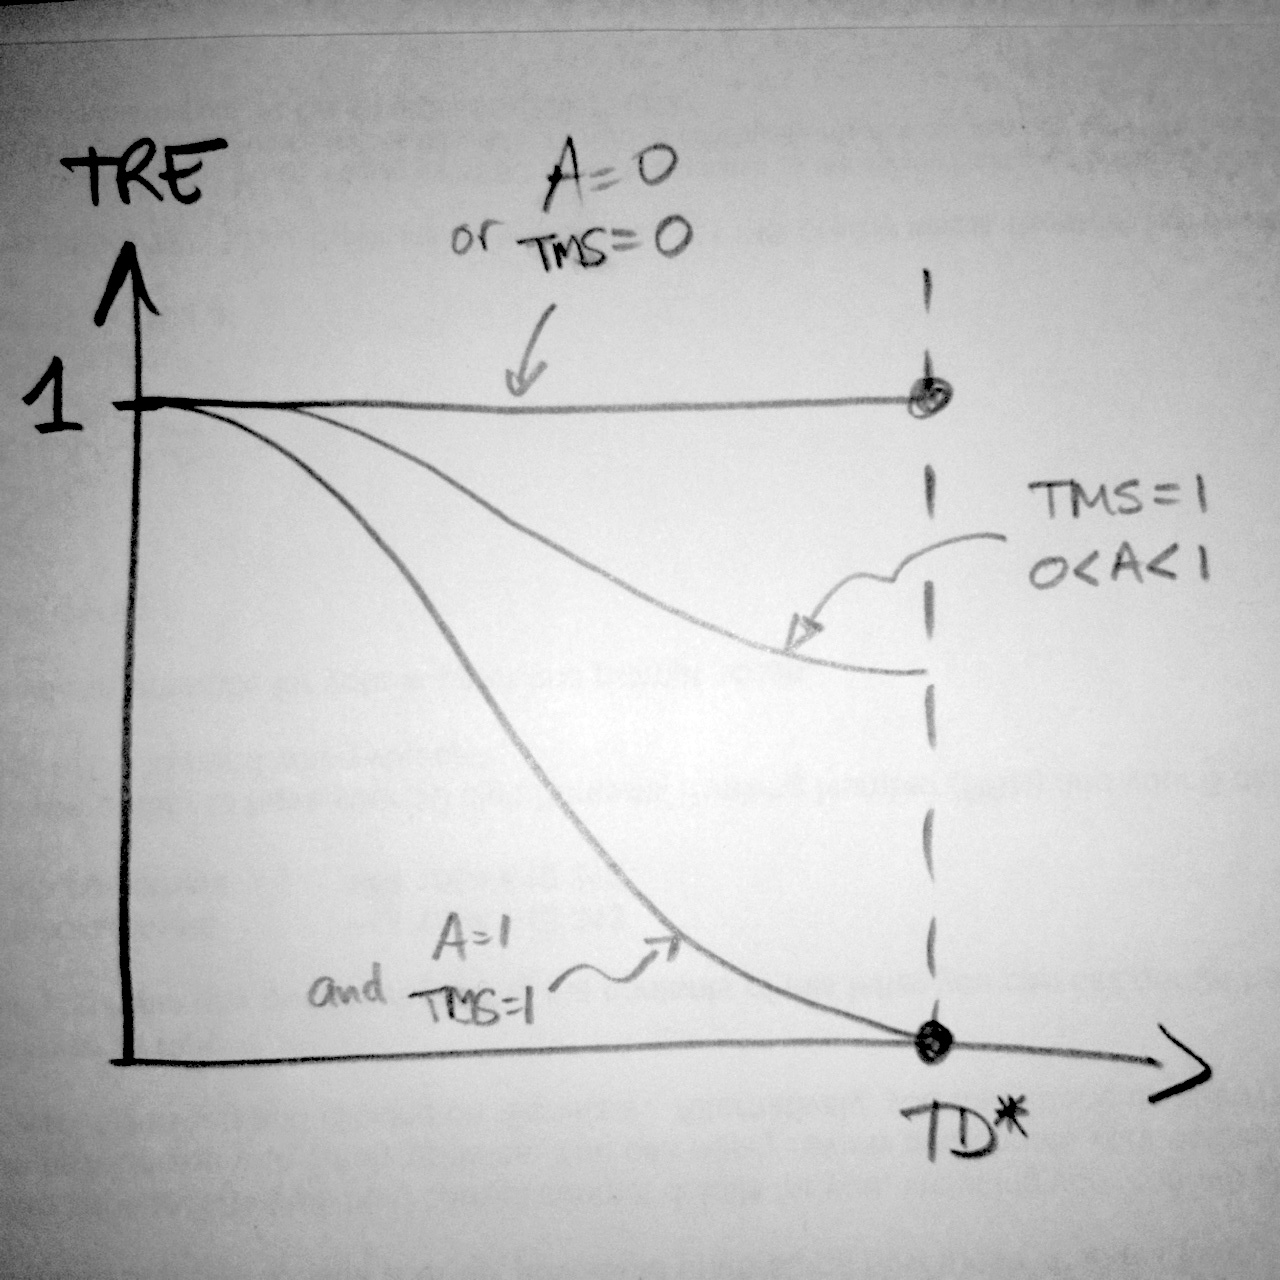
\includegraphics[angle=0,width=0.5\textwidth]{figures/TRE.JPG}
\caption{Treatment reduction effect.}
\label{fig:TRE}
\end{figure}

The infectivity curve before treatment ($IC$) is thus modified into an infectivity curve during treatment ($IC^{treat}$):
$$IC^{treat}(t,\tau)= IC(t)\times TRE(A,TMS,\tau)  $$

For curable STIs, cure is achieved by assessing the value of a random variable with a Bernoulli distribution 
$$Cure \sim \mathrm{Bern}(TRE(TD^*)) $$

If $Cure=1$, the STI is cured. If $Cure=0$ the infectivity curve is set back, as if $TRE=1$.




%%%%%%%%%%%%%%%%%%%%%%%%%%%%%%%%%%%%%%%%%%%%%
%%%%%%%%%%%%%%%%%%%%%%%%%%%%%%%%%%%%%%%%%%%%%

\section{Simulation}

This section gives a high-level description of how the simulation can be run. 

\subsection{Calibration}

\subsubsection{Response variable of the Model to be calibrated}

This agent-based model has many model parameters and calibrating as much data as possible before running simulation is desirable. Table \ref{tab:calibration} gives an example of data needed to fit some of the model parameters.

\begin{table}[htdp]
\caption{Response variables to be calibrated}
\begin{center}
\begin{tabular}{lll}

\hline
\textbf{Category} & \textbf{Target Quantity} & \textbf{Parameters} \\

\hline
Demographic  &  Age structure & Birth rates, death rates (Weibull parameters)\\
 & & (STI prevalence when HIV modelled)\\
\hline
Partnerships  &  Ratio \#singles/total population  &  Formation/dissolution rates and preferences \\
  &  Age gaps &   Formation/dissolution rates and preferences  \\
  &  Spousal ratio & Spousal preferences \\
 & & (STI prevalence when HIV modelled)\\
\hline
STIs	& Global prevalence & Demographics, partnerships,\\
	& Prevalence by risk group & STI infectivity/susceptibility,\\
	& Prevalence by age & CSW and sex behaviour\\
\hline
\end{tabular}
\end{center}
\label{tab:calibration}
\end{table}


The objective function to minimize can be expressed as $F(X)$, with $X$ is the vector of all parameters to be calibrated such that the response variables are the closest to their respective target. For example:
\begin{eqnarray*}
F(X) & =&\,\omega_{AD}(AgeDist - target_{AD})^2 \\
& & + \omega_{PR}(PartnerRatio - target_{PR})^2 \\
& & + \omega_{AG}(AgeGap - target_{AG})^2 \\
& & +\sum_s \omega_{TP}(STItotPrev_s-target_{TP,s})^2 \\
& & +\sum_s \omega_{RGP}(STIRiskGrpPrev_s-target_{RGP,s})^2\\
& & +\sum_s \omega_{AP}(STIAgePrev_s-target_{AP,s})^2
\end{eqnarray*}
with $\omega$ calibration weights. 

We search $X^*$ such that $F(X^*)=\min_{X\in \mathcal{A}} F(X)$, where $\mathcal{A}$ is the parameter space delimited by predefined lower and upper bounds.


\subsection{Simulations}

The high-level steps below are a suggestion to perform an epidemiological analysis using this agent-based model:

\begin{enumerate}
\item start with initial population, no partnerships, no STI
\item run simulation long enough such that the partnership dynamics are in a steady state
\item calibration to target demographic and partnership data should be performed at that step
\item introduce STI into the population and make epidemiological analysis.
\end{enumerate}


\section{Appendix}
\subsection{Pseudo-beta shape function} \label{sec:pseudobeta}

For infectivity curves associated with STIs of limited duration, the shape function was inspired from the beta distribution density (because it has a bounded support).
$$\mathcal{B}(x,a,b) = x^{a-1}(1-x)^{b-1}/C$$
where $C$ is the normalizing constant such that the maximum value of $\mathcal{B}$ is 1 on the interval [0;1]:
$$C=\left(\frac{a-1}{a+b-2}\right)^{a-1}\left(\frac{b-1}{a+b-2}\right)^{b-1}$$
It is assumed that for any $a,b>1$ and  $x<0$ and $x>1$ we have $\mathcal{B}(x,a,b)=0$.
The maximum of $\mathcal{B}$ is reached at $x_{max}=(a-1)/(a+b-2)$.


\newpage
\bibliographystyle{vancouver}
\bibliography{papers.bib}
\end{document}

